% Niniejszy plik stanowi przykład formatowania pracy magisterskiej na
% Wydziale MIM UW.  Szkielet użytych poleceń można wykorzystywać do
% woli, np. formatujac wlasna prace.
%
% Zawartosc merytoryczna stanowi oryginalnosiagniecie
% naukowosciowe Marcina Wolinskiego.  Wszelkie prawa zastrzeżone.
%
% Copyright (c) 2001 by Marcin Woliński <M.Wolinski@gust.org.pl>
% Poprawki spowodowane zmianami przepisów - Marcin Szczuka, 1.10.2004
% Poprawki spowodowane zmianami przepisow i ujednolicenie 
% - Seweryn Karłowicz, 05.05.2006
% Dodanie wielu autorów i tłumaczenia na angielski - Kuba Pochrybniak, 29.11.2016

% dodaj opcję [licencjacka] dla pracy licencjackiej
% dodaj opcję [en] dla wersji angielskiej (mogą być obie: [licencjacka,en])
\documentclass[licencjacka,en]{pracamgr}

\usepackage{times}
% \usepackage[marginparwidth=75pt]{geometry}
% Optional math commands from https://github.com/goodfeli/dlbook_notation.
\input{math_commands.tex}

\usepackage{hyperref}
\usepackage{url}
\usepackage{times}
% additional packages
\usepackage{graphicx}
\usepackage{xspace}
\usepackage[capitalise]{cleveref}
\usepackage{wrapfig}
\usepackage{multirow}
\usepackage{array}
\usepackage{booktabs}
\usepackage{tabularray}
\usepackage{amsmath}
\usepackage{algorithm}
\usepackage{algpseudocode}
\usepackage{subcaption}
\usepackage{cleveref}
\usepackage{xspace}
\usepackage{xcolor}
\usepackage{fontawesome5}
\usepackage{natbib}  % or \usepackage{biblatex} if you prefer biblatex
\bibliographystyle{plainnat}  % or another style of your choice

\usepackage{xargs}                      % Use more than one optional

\newcommand{\fix}{\marginpar{FIX}}
\newcommand{\new}{\marginpar{NEW}}
\newcommand{\isb}{I\textsuperscript{2}SB}
\newcommand{\isbs}{I\textsuperscript{2}SBs}
\newcommand{\todo}[1]{\textcolor{black}{#1}}
\newcommand{\note}[1]{\textcolor{orange}{#1}}
\newcommand{\method}[1]{EquiDiff}  % Equivariant Diffusion Sampling
\newcommand{\framework}[1]{Invariants}  % Invariant Images
% DIVA (Diverse Invariant Visual Analysis)
% GUIDE (Generative Understanding of Invariant Domains via Equivariance)

\newcommand{\diff}{\mathrm{d}}
\newcommand{\scoret}{\nabla_{\mathbf{x}_t} \log{p(\mathbf{x}_t, t)}}
\newcommand{\scoren}{\nabla_{\mathbf{x}_n} \log{p(\mathbf{x}_n, n)}}
\newcommand{\scoretwithcond}{\nabla_{\mathbf{x}_t} \log{p(\mathbf{x}_t, t \mid \mathbf{y})}}
\newcommand{\scorenwithcond}{\nabla_{\mathbf{x}_n} \log{p(\mathbf{x}_n, n \mid \mathbf{y})}}
\newcommand{\scoretcond}{\nabla_{\mathbf{x}_t} \log{p(\mathbf{y} \mid \mathbf{x}_t, t)}}
\newcommand{\scorencond}{\nabla_{\mathbf{x}_n} \log{p(\mathbf{y} \mid \mathbf{x}_n, n)}}
\newcommand{\nonlscoret}{\nabla_{\mathbf{x}_t} \log \boldsymbol{\Psi}(\mathbf{x}_t, t)}
\newcommand{\nonlhscoret}{\nabla_{\mathbf{x}_t} \log \widehat{\boldsymbol{\Psi}}(\mathbf{x}_t, t)}
\newcommand{\boldpsi}{\boldsymbol{\Psi}}
\newcommand{\boldhatpsi}{\widehat{\boldsymbol{\Psi}}}
\newcommand{\boldpsistar}{\boldsymbol{\Psi}^*}
\newcommand{\boldhatpsistar}{\widehat{\boldsymbol{\Psi}}^*}

\DeclareFontFamily{U}{matha}{\hyphenchar\font45}
\DeclareFontShape{U}{matha}{m}{n}{
      <5> <6> <7> <8> <9> <10> gen * matha
      <10.95> matha10 <12> <14.4> <17.28> <20.74> <24.88> matha12
      }{}
\DeclareSymbolFont{matha}{U}{matha}{m}{n}

\DeclareMathSymbol{\Lt}{3}{matha}{"CE}
\DeclareMathSymbol{\Gt}{3}{matha}{"CF}

% \pdfminorversion=7
% \pdfobjcompresslevel=0

% Dane magistranta:
\autor{Bartłomiej Sadlej}{429589}

\title{EquiDiff: Generative Exploration of Neural Network Invariant Sets through Diffusion-Based Sampling}
\titlepl{EquiDiff: Generatywna Eksploracja Zbiorów Niezmienniczych Sieci Neuronowych przez Próbkowanie Oparte na Dyfuzji}

\kierunek{Machine Learning}

% Praca wykonana pod kierunkiem:
\opiekun{prof. dr hab. inż. Przemysław Biecek\\
  Wydział Matematyki Informatyki i Mechaniki\\
  }

% miesiąc i~rok:
\date{September 2025}

%Podać dziedzinę wg klasyfikacji Socrates-Erasmus:
\dziedzina{ 
11.4 Sztuczna inteligencja\\ 
11.3 Informatyka\\
11.1 Matematyka
}

%Klasyfikacja tematyczna wedlug ACM (informatyka)
\klasyfikacja{I. Computing Methodologies\\
  I.2 Artificial Intelligence\\
  I.2.6 Learning\\
  I.2.10 Vision and Scene Understanding\\
  I.4 Image Processing and Computer Vision\\
  I.4.8 Scene Analysis
}

% Słowa kluczowe:
\keywords{explainable AI, generative models, diffusion models, invariant sets, level sets, neural network interpretability, mechanistic interpretability, sparse autoencoders, visual explanations, counterfactual generation, score-based generative models}

% Tu jest dobre miejsce na Twoje własne makra i~środowiska:
\newtheorem{defi}{Definicja}[section]

% koniec definicji

\begin{document}
\maketitle

%tu idzie streszczenie na strone poczatkowa
\begin{abstract}
Understanding the decision-making process of deep neural networks is an active area of research in machine learning. Current state of the art methods focus on finding human-interpretable concepts or features that influence predictions in known data samples. However, we argue that this approach is limited in its ability to provide a comprehensive understanding of model behavior due to vast unexplored regions of the data manifold, not present in investigated datasets, which can potentially lead to the same predictions. The main contribution of this work is paradigm shift from traditional explainable AI (XAI) methods where we find human-interpretable features in known data to generative XAI methods that synthesize new samples. This work first introduces new framework \textit{\framework{}} - a theoretical backbone for generative XAI methods and then proposes new method \method which an efficient implementation of this framework. Evaluation of this methon on popular models such as ResNet-50 or Sprase AutoEncoders (SAE) points out significant limitations of current XAI methods.

This work is a continuation of pioneering work on Generative Explainable AI (XAI) \citep{sobieski2024rethinkingvisualcounterfactualexplanations} published at International Conference on Learning Representations 2025 and introduces a novel framework of \framework{} - sets of data points that yield identical predictions under a given model, thereby establishing an equivalence relation. Our method \method{} allows for sampling meaningful and diverse high quality realistic examples from these invariant sets and as a result opens new possibilities for  evaluating existing explainability methods on unknown data - simulating the real world, and fully preventing training data leaks by generating synthetic samples. 
\end{abstract}

\tableofcontents

\chapter{Introduction}\label{r:introduction}

The remarkable success of deep neural networks in computer vision has been accompanied by an equally pressing need to understand their decision-making processes. As these models are deployed in critical applications ranging from medical diagnosis to autonomous driving, the ability to explain and interpret their behavior becomes paramount for building trust, ensuring fairness, and identifying potential failure modes.

Current explainable AI (XAI) methods have made significant strides in providing insights into model behavior through various approaches including saliency maps \citep{simonyan2014deepinsideconvolutionalnetworks}, concept activation vectors \citep{kim2018interpretabilityfeatureattributionquantitative}, and gradient-based attribution methods \citep{sundararajan2017axiomaticattributiondeepnetworks}. However, these approaches share a fundamental limitation: they primarily operate within the confines of known training data or slight perturbations thereof, leaving vast regions of the input manifold unexplored.

More recent advancements that expand the scope of interpretability try to address those limitations. Approaches such as Rate-Distortion Explanation (RDE) frameworks systematically perturb input signals across diverse data modalities to identify truly relevant features, thereby moving beyond local sensitivity \citep{Kolek2022}. These frameworks also explicitly aim for in-distribution interpretability by leveraging generative models like in-painting GANs, thereby guarding against explanations corrupted by evaluations in undeveloped or unrealistic regions of the model's function. Similarly, new techniques for interpreting deep generative models (GANs) enable the identification of human-understandable concepts within latent spaces, allowing for interactive image generation and editing. This actively explores the input manifold by creating new data, offering insights into how realistic images are composed from deep representations. \citep{zhou2022interpretinggenerativeadversarialnetworks, Karimi2022}

Furthermore, XAI is seeing a shift towards building transparency into models from the outset, often referred to as "interpretable-by-design" methods \citep{Karimi2022, Holzinger2022a}. Research into interpretable reinforcement learning via programmatic policies aims to train policies in the form of human-readable programs (e.g., decision trees, state machines), which are inherently more interpretable, verifiable, and robust than traditional deep neural network policies \citep{inbook, Inala2020Synthesizing, verma2019programmaticallyinterpretablereinforcementlearning}. Likewise, Explainable Neural-Symbolic Learning (X-NeSyL) represents another design-based approach, fusing deep learning representations with expert knowledge graphs to encourage neural networks to learn structures akin to human expert reasoning, ensuring interpretability is embedded throughout the training process \citep{D_az_Rodr_guez_2022, karimi2020algorithmicrecoursecounterfactualexplanations}.

These advancements align with what is sometimes referred to as "RED XAI" – a model-centric culture focused on questioning models, extracting knowledge, spotting, and fixing bugs, and ultimately improving the reliability and safety of AI systems \citep{10.5555/3692070.3692231}. This perspective is critical for using explanations not just to justify decisions, but to drive model development and verification \citep{Tsai2022}. This includes attributing importance to feature interactions and groups, which can then be used to directly improve model generalization or to distill complex models into simpler forms, often validated through "reality checks" \citep{Singh2022}
\section{Motivation and Problem Statement}

Consider a trained image classifier that correctly identifies both a standard photograph of a dog and a highly stylized artistic rendering of the same animal. Traditional XAI methods would analyze these two specific instances, potentially identifying common features like shape or texture patterns. However, they would miss the broader question: what other visual representations would this model also classify as a dog with the same confidence?

When we say "a dog with the same confidence," we mean something far more profound and potentially disturbing than might initially appear. We are not merely talking about different breeds of dogs, or dogs photographed from different angles, or even dogs rendered in different artistic styles. We are talking about the complete universe of visual patterns—no matter how bizarre, abstract, or seemingly unrelated to dog anatomy—that trigger identical neural responses in the classifier's decision-making apparatus. This could include a Jackson Pollock painting with just the right splatter of paint, a close-up photograph of tree bark with particular texture patterns, a geometric arrangement of colored pixels that bears no resemblance whatsoever to any living creature, or even a photograph of a kitchen appliance that happens to contain the precise combination of edges, curves, and color distributions that the model has learned to associate with "dog-ness." The classifier would assign these wildly disparate inputs exactly the same probability score—perhaps 0.8347 for "dog"—despite their complete lack of semantic relationship to actual dogs.

This question is not merely academic but reveals a fundamental blindness in our understanding of machine learning models. Traditional explainable AI methods focus on the narrow slice of reality represented in training datasets, leaving vast territories of the input manifold completely unexplored and potentially harboring unexpected model behaviors. The robustness implications are staggering: if a model can be fooled into seeing a dog in a random arrangement of geometric shapes with the same confidence as it sees a dog in an actual photograph of a Golden Retriever, what does this say about its reliability in real-world deployment? The bias detection possibilities are equally concerning—systematic patterns within these datasets might reveal that the model has learned to associate certain irrelevant features (perhaps related to image compression artifacts, camera settings, or demographic markers in the background) with specific classes, perpetuating hidden biases that would never be discovered through traditional dataset analysis. For fairness evaluation, understanding these equivalence classes becomes critical: if the model makes identical predictions for inputs that vary along protected attributes while maintaining other spurious correlations, we need to map these relationships to ensure equitable treatment. Finally, the structure of these datasets provides unprecedented insight into how models generalize beyond their training distribution—revealing whether generalization relies on semantically meaningful features or on arbitrary statistical regularities that happen to correlate with class labels in the training data.

\section{Our Approach: Generative Explainable AI}

This thesis introduces a paradigm shift from traditional interpolative XAI methods to a generative approach. Instead of analyzing existing data points, we propose synthesizing new, meaningful examples that preserve model predictions, thereby exploring the \textit{Invariant Set} -- the complete collection of inputs that yield identical outputs under a given objective function.

Our method, \method{} (Equivariant Diffusion Sampling), combines score-based generative models with classifier guidance to sample high-quality, diverse images from these invariant sets. By leveraging the powerful generative capabilities of diffusion models, we can explore regions of the input space that may never have been encountered during training, providing a more comprehensive understanding of model behavior.

Figure~\ref{fig:1_teaser} illustrates the conceptual distinction between our approach and current XAI methods. While traditional methods focus on explaining decisions within known data boundaries, generative XAI does not have this limitation and can explore the broader space of possible inputs that lead to the same predictions.

\begin{figure}[h]
\centering
\includegraphics[width=0.8\linewidth]{figures/main/teaser1.png}
\caption{Conceptual comparison between traditional XAI methods and Generative XAI. Traditional methods analyze known data samples (left), while our approach synthesizes diverse examples from the invariant set that yield identical predictions (right).}
\label{fig:1_teaser}
\end{figure}

\section{Contributions}

This thesis makes three key contributions to the field of explainable AI, as outlined in the abstract and detailed in Chapter~\ref{r:method}:

The first contribution represents a \textbf{paradigm shift from traditional explainable AI methods} that analyze human-interpretable features in known data samples to generative XAI methods that synthesize new samples. This fundamental change in perspective allows for exploration of vast regions of the input manifold that remain unexplored by current approaches, providing a more comprehensive understanding of model behavior beyond the confines of training datasets.

The second contribution introduces the \textbf{\framework{} framework} -- a novel theoretical backbone for generative XAI methods. This framework provides formal mathematical definitions of invariant sets and establishes their properties as equivalence relations, offering a rigorous foundation for understanding and generating diverse examples that yield identical model predictions.

The third contribution presents \textbf{\method{}} -- an efficient algorithmic implementation of the \framework{} framework. This method combines score-based diffusion models with guided sampling to generate high-quality, diverse examples from invariant sets, enabling practical application of the theoretical framework to real-world neural network analysis and interpretation.

These contributions are comprehensively detailed and evaluated in Chapter~\ref{r:method}, where we present both the theoretical foundations and empirical validation of our approach.

\section{Thesis Organization}

The remainder of this thesis is structured to provide a comprehensive exploration of our generative explainable AI approach. Chapter~\ref{r:related_work} reviews the relevant literature across explainable AI methods, generative modeling, and diffusion models, establishing the theoretical foundation for our work. Chapter~\ref{r:method} presents our core theoretical framework and details the \method{} algorithm, providing the mathematical foundation for invariant set generation and the practical implementation of our approach.

Chapter~\ref{r:experiments} presents a comprehensive experimental evaluation demonstrating the effectiveness of our method across multiple neural network analysis paradigms, from individual neuron activation to complete classifier output preservation. Chapter~\ref{r:applications} explores practical applications of our framework in real-world scenarios, while Chapter~\ref{r:discussion} discusses the broader implications of our work, current limitations, and directions for future research. Chapter~\ref{r:conclusion} synthesizes our contributions and their significance for the field of explainable AI.

\chapter{Related Work}\label{r:related_work}

This chapter reviews the relevant literature across several interconnected areas that form the foundation of our work. We begin with an overview of explainable AI methods, followed by background on score-based generative models, conditional generation techniques, and related work on activation maximization and concept discovery.

\section{Explainable Artificial Intelligence}

The field of explainable AI has evolved rapidly in response to the growing complexity and opacity of modern deep learning models. Current approaches can be broadly categorized into several paradigms:

\subsection{Attribution Methods}

Attribution methods aim to identify which input features are most important for a model's prediction in a form of a heatmap. Gradient-based methods like Integrated Gradients \citep{sundararajan2017axiomaticattributiondeepnetworks} and GradCAM \citep{8237336} compute the gradient of the output with respect to input features to determine importance scores. While computationally efficient, these methods are limited to local explanations around specific data points and can be sensitive to model architecture and input preprocessing.

Perturbation-based methods such as LIME \citep{ribeiro2016whyitrustyou} and SHAP \citep{lundberg2017unifiedapproachinterpretingmodel} evaluate feature importance by measuring how predictions change when features are masked or altered. These methods provide more model-agnostic explanations but are computationally expensive and may not capture complex feature interactions.

\subsection{Concept-Based Methods}

Concept-based explainability methods attempt to understand models in terms of human-interpretable concepts. Concept Activation Vectors (CAVs) \citep{kim2018interpretabilityfeatureattributionquantitative} learn linear directions in activation space that correspond to human-defined concepts. Network Dissection \citep{bau2017networkdissectionquantifyinginterpretability} automatically discovers concepts by correlating individual neurons with semantic segmentation labels.

More recent work has focused on discovering concepts automatically without human supervision. ACE (Automatic Concept Extraction) \citep{ghorbani2019automaticconceptbasedexplanations} uses unsupervised segmentation to identify important concepts, while TCAV (Testing with CAVs) \citep{kim2018interpretabilityfeatureattributionquantitative} provides statistical significance testing for concept importance.

\subsection{Counterfactual Explanations}

Counterfactual explanations answer the question "What would need to change for the model to make a different prediction?" This paradigm has gained popularity due to its intuitive nature and practical utility. Although earlier work has explored generative models for visual counterfactual explanations, \citep{sobieski2024rethinkingvisualcounterfactualexplanations} advanced this direction in a way that directly inspired our approach. Our method is, to our knowledge, the first to combine high-quality results with almost real-time performance.

In counterfactual methods, the objective is generally defined as finding the smallest possible changes to an input that alter the model’s decision—for example, modifying a few pixels in an image so that the predicted class changes. In contrast, our goal is to generate diverse examples that preserve the original prediction.

\section{Score-Based Generative Models}\label{sec:sgm_background}

Score-based generative models (SGMs) have emerged as a powerful framework for high-quality image generation. Following the seminal work of \citep{song2021scorebasedgenerativemodelingstochastic}, these models can be understood through the lens of stochastic differential equations (SDEs).

\subsection{Mathematical Foundation}

The core idea behind SGMs is to transform samples from a complex data distribution $p_0$ (e.g. natural images) to a simple noise distribution $p_1$ (typically Gaussian) through a forward diffusion process and then learn to reverse this transformation. The forward SDE is given by:

\begin{equation}
\diff \mathbf{x}_t = \mathbf{f}(\mathbf{x}_t, t) \diff t + g(t) \diff \mathbf{w}_t
\label{eq:forward_sde}
\end{equation}

where $\mathbf{x}_t$ represents the noisy version of a clean image at time $t \in [0, 1]$, $\mathbf{f}(\mathbf{x}_t, t)$ is the drift coefficient, $g(t)$ is the diffusion coefficient, and $\mathbf{w}_t$ is a Wiener process.

The corresponding reverse SDE, which enables generation, is:

\begin{equation}
\diff \mathbf{x}_t = [\mathbf{f}(\mathbf{x}_t, t) - g(t)^2 \nabla_{\mathbf{x}_t} \log p_t(\mathbf{x}_t)] \diff t + g(t) \diff \bar{\mathbf{w}}_t
\label{eq:reverse_sde}
\end{equation}

The key term $\nabla_{\mathbf{x}_t} \log p_t(\mathbf{x}t)$ is the score function, which must be learned by a neural network $\mathbf{s}{\boldsymbol{\theta}}(\mathbf{x}_t, t)$, since it cannot be computed analytically without access to the final, fully denoised image.

\subsection{Training and Sampling}

Score networks are typically trained using denoising score matching \citep{6795935, song2020generativemodelingestimatinggradients}:

\begin{equation}
\mathcal{L}(\boldsymbol{\theta}) = \mathbb{E}_{t, \mathbf{x}_0, \boldsymbol{\epsilon}} \left[ \lambda(t) \|\mathbf{s}_{\boldsymbol{\theta}}(\mathbf{x}_t, t) - \boldsymbol{\epsilon}\|_2^2 \right]
\label{eq:score_matching_loss}
\end{equation}

where $\mathbf{x}_t = \alpha(t)\mathbf{x}_0 + \sigma(t)\boldsymbol{\epsilon}$ with $\boldsymbol{\epsilon} \sim \mathcal{N}(0, \mathbf{I})$, and $\lambda(t)$ is a weighting function.

During sampling, we start from pure noise $\mathbf{x}_1 \sim \mathcal{N}(0, \mathbf{I})$ and integrate the reverse SDE using numerical solvers, with the learned score function $\mathbf{s}_{\boldsymbol{\theta}}$ approximating the true score.

\section{Conditional Generation and Classifier Guidance}

Conditional generation extends SGMs to produce samples conditioned on additional information $\mathbf{y}$, such as class labels or other attributes. The conditional score function can be decomposed using Bayes' theorem:

\begin{equation}
\nabla_{\mathbf{x}_t} \log p(\mathbf{x}_t \mid \mathbf{y}, t) = \nabla_{\mathbf{x}_t} \log p(\mathbf{x}_t, t) + \nabla_{\mathbf{x}_t} \log p(\mathbf{y} \mid \mathbf{x}_t, t)
\label{eq:conditional_score}
\end{equation}

\subsection{Classifier Guidance}

Classifier guidance \citep{dhariwal2021diffusionmodelsbeatgans} implements conditional generation by training an auxiliary time-dependent classifier $p_{\boldsymbol{\phi}}(\mathbf{y} \mid \mathbf{x}_t, t)$ on noisy images and incorporating its gradients into the sampling process:

\begin{equation}
\tilde{\mathbf{s}}_{\boldsymbol{\theta}}(\mathbf{x}_t, t, \mathbf{y}) = \mathbf{s}_{\boldsymbol{\theta}}(\mathbf{x}_t, t) + s \cdot \nabla_{\mathbf{x}_t} \log p_{\boldsymbol{\phi}}(\mathbf{y} \mid \mathbf{x}_t, t)
\label{eq:classifier_guidance}
\end{equation}

where $s$ is the guidance scale that controls the trade-off between sample quality and diversity.

\subsection{Limitations of Standard Classifier Guidance}

While effective for class-conditional generation, standard classifier guidance has several limitations for our application:

\begin{enumerate}
\item \textbf{Limited Optimization Steps}: Guidance is applied only at discrete points along the denoising trajectory, due to the fixed number of diffusion steps, which can constrain the precision of conditioning.

\item \textbf{Latent Space Considerations}: Many state-of-the-art diffusion models operate in latent space, requiring careful alignment of the conditioning signal with the model’s latent representation.

\item \textbf{Objective Function Alignment}: In its standard form, classifier guidance is tailored for classification objectives (predicting $p(y \mid x)$). While the conditioning variable $y$ can, in principle, represent a wide range of targets beyond class labels, adapting it to arbitrary objective functions may require additional formulation effort.
\end{enumerate}

These limitations motivate our approach, which we detail in Chapter~\ref{r:method}.

\section{Inverse Problems and Posterior Sampling}

Recent work has explored the use of diffusion models as priors for solving inverse problems in image restoration \citep{song2023pseudoinverse, chung2024diffusionposteriorsamplinggeneral}. The general inverse problem can be formulated as:

\begin{equation}
\mathbf{y} = \mathcal{A}(\mathbf{x}) + \boldsymbol{\epsilon}
\label{eq:inverse_problem}
\end{equation}

where $\mathcal{A}$ is a (possibly nonlinear) forward operator, $\mathbf{x}$ is the unknown signal, $\mathbf{y}$ is the observed measurement, and $\boldsymbol{\epsilon}$ is an additive noise term, which may follow different distributions (e.g., Gaussian, Poisson) and can exhibit nontrivial covariance structures.

\citep{chung2024diffusionposteriorsamplinggeneral} showed that diffusion models can address nonlinear inverse problems for arbitrary differentiable forward systems by incorporating the measurement likelihood into the reverse SDE. Their framework accommodates various noise models, including Gaussian and Poisson. This is particularly relevant to our approach, as neural network predictions can be interpreted as nonlinear measurements of the input image.

\subsection{Diverse Posterior Sampling}

More recently, \citep{cohen2024posteriorsamplingmeaningfuldiversity} extended inverse problem solvers to generate diverse solutions rather than a single best estimate. This paradigm shift from point estimation to posterior sampling aligns closely with our goal of generating new data samples.

\section{Activation Maximization and Feature Visualization}

Activation maximization techniques attempt to synthesize inputs that maximally activate specific neurons or model outputs \citep{erhan2009visualizing, mordvintsev2015deepdream}. The basic approach optimizes an input image $\mathbf{x}$ to maximize an objective function $\mathcal{L}(\mathbf{x})$:

\begin{equation}
\mathbf{x}^* = \arg\max_{\mathbf{x}} \mathcal{L}(\mathbf{x}) - \lambda \mathcal{R}(\mathbf{x})
\label{eq:activation_maximization}
\end{equation}

where $\mathcal{R}(\mathbf{x})$ is a regularization term to encourage natural-looking images.

However, activation maximization methods often produce unrealistic images accompanied by high-frequency artifacts that are imperceptible to humans yet strongly activate neurons \citep{shinkle2025visualizingcontrollingcorticalresponses, nanfack2023adversarialattacksinterpretationneuron, zhu2025representationunderstandingactivationmaximization}. To address this, various regularization techniques have been proposed, including total variation penalties, which encourage smoother and more coherent outputs \citep{mahendran2014understandingdeepimagerepresentations}, and frequency domain constraints that reduce high-frequency noise and improve interpretability \citep{olah2017feature}.

\subsection{Limitations and Relationship to Our Work}

Although activation maximization shares the goal of understanding model behavior through synthetic inputs, it differs fundamentally from our approach.

\begin{enumerate}
\item \textbf{Single Solution vs. Diverse Sets}: Activation maximization typically finds one optimal input, while we aim to generate a set of new data points.

\item \textbf{Maximum Activation vs. Preserved Predictions}: Activation maximization seeks to maximize responses while we preserve specific prediction values.

\item \textbf{Quality Issues}: Traditional activation maximization often produces unrealistic images, while our diffusion-based approach leverages strong visual priors.
\end{enumerate}

\section{Concept Discovery and Spurious Feature Detection}

Understanding what concepts neural networks learn has been an active area of research. \citep{Lapuschkin_2019} developed SpRAy, an automatic pipeline for exploring shortcuts and biases learned by models, often referred to as "Clever Hans" effects \citep{pfungst1911cleverHans}. \citep{neuhaus2023spuriousfeatureslargescale} investigates methods for automatically finding spurious features in training data.

Recent work by \citep{dreyer2025mechanisticunderstandingvalidationlarge} addresses the question of what concepts were learned by models and where in the training data they were present. However, \citep{leask2025sparse} argues that automatically discovered concepts may lack atomicity and completeness.

Our work complements this line of research by exploring the space of inputs that preserve predictions, potentially revealing spurious correlations and biases that may not be apparent from training data analysis alone.

\section{Detection of Synthetic Images}

As generative models become increasingly sophisticated, detecting synthetic images has become an important research area. Modern architectures using resampling operations (upsampling, downsampling, interpolation) introduce specific periodic correlations between pixels that are rarely present in natural images \citep{Popescu2005ExposingDF}.

Recent advances in synthetic image detection \citep{zhang2019detectingsimulatingartifactsgan, wang2023dirediffusiongeneratedimagedetection, zhang2023diffusion} have achieved near-perfect accuracy on images generated by GANs and diffusion models by analyzing frequency domain artifacts.

While our goal is not to evade detection methods, we acknowledge that our images are synthetic. Drawing on insights from this literature, we aim for the Fourier spectrum of our generated images to match that of real images, ensuring that model predictions are not driven by imperceptible frequency artifacts but by signal patterns consistent with natural image statistics.

\section{Gap in Current Literature}

Despite significant advances in XAI, a fundamental gap remains: current methods primarily analyze known training data and model behavior on observed inputs. This leaves vast regions of the input manifold unexplored, potentially missing important insights about model behavior.

Our work addresses this gap by introducing a principled framework for exploring the space of alternative inputs that yield identical predictions. By leveraging powerful generative models, we sample from regions of the input space that were observed during training but represent continuous interpolations and variations of the training data, providing a more comprehensive understanding of model behavior within the learned data manifold.
\chapter{Method}\label{r:method}

This chapter presents our theoretical framework and algorithmic approach for generating \framework{}. We begin with formal definitions that relate our concept to classical level sets from differential topology \citep{lee2013smooth,milnor1965topology,fort2017gaussian}, establish our theoretical foundation, detail our algorithm, and conclude with implementation specifics and quality assurance measures.

\begin{figure}[h]
\centering
\includegraphics[width=\linewidth]{figures/main/invariant_framework_combined.pdf}
\caption{Demonstration of the Invariant Framework on a 2D Concentric Circles Dataset.
(a) Training dataset with 1,500 samples classified by their position relative to a unit circle (dashed line). Blue points represent the outer class, pink points the inner class.
(b) Learned decision boundary and prediction probability heatmap from a 3-layer MLP (test accuracy: 0.983). The black contour shows the 0.5 decision boundary.
(c-e) Invariant sets for three query points (black stars) with prediction values p. Orange points represent all input locations that yield identical predictions under the trained model, demonstrating the equivalence relation established by the model's output. The invariant sets approximate level curves of the learned decision function, revealing the geometric structure of the model's decision space.}
\label{fig:teaser}
\end{figure}

\section{Problem Formulation}
We formulate the problem of finding invariant sets (IS) as discovering members of an equivalence relation. Given a neural network with parameters $\boldsymbol{\theta}$ and objective function $\mathcal{L}_{\boldsymbol{\theta}}:\mathbb{R}^n \rightarrow \mathbb{R}^m$, and a query point $\mathbf{x^*}$, we define the invariant set as:
\begin{equation}
  \mathbf{IS}(\mathbf{x^*}) = \{ \mathbf{x} \in \mathbb{R}^n : \mathcal{L}_{\boldsymbol{\theta}}(\mathbf{x}) = \mathcal{L}_{\boldsymbol{\theta}}(\mathbf{x^*}) \}
  \label{eq:is}
\end{equation}
We use the notation $\mathbf{x^*} \sim_{\mathcal{L}_{\boldsymbol{\theta}}} \mathbf{x}$ to denote that two elements $\mathbf{x^*}$ and $\mathbf{x}$ belong to the same invariant set under the equivalence relation defined by $\mathcal{L}_{\boldsymbol{\theta}}$.

The objective function $\mathcal{L}_{\boldsymbol{\theta}}$ can represent various neural network components: a single neuron's activation, class logits for one or multiple classes, or any differentiable function for which gradients can be computed. While adversarial examples can be viewed as specific perturbations that may belong to invariant sets under certain conditions \citep{szegedy2014intriguingpropertiesneuralnetworks}, our goal is fundamentally different: we seek to sample from the intersection of the invariant set with the natural data manifold, ensuring realism by construction.

To achieve this, we utilize a trained diffusion model, specifically LightningDIT \citep{yao2025vavae} \citep{yao2024fasterdit}, which excels at generating high-quality images while maintaining the mathematical constraints of invariant set membership. The diversity of examples emerges naturally from exploring different regions of this manifold intersection.


\section{Guided Iterative Optimization with Latent Diffusion Models}

Our algorithm integrates signals from the neural network function $f_{\boldsymbol{\theta}}:\mathbb{R}^{W \times H} \rightarrow \mathbb{R}^m$ through a scalar loss function $\ell: \mathbb{R}^m \times \mathbb{R}^m \rightarrow \mathbb{R}$ to conditionally synthesize images from invariant sets. Given a target output $\mathbf{y^*} = f_{\boldsymbol{\theta}}(\mathbf{x^*})$, we define our objective as:
\begin{equation}
\mathcal{L}(\mathbf{x}) = \ell(f_{\boldsymbol{\theta}}(\mathbf{x}), \mathbf{y^*})
\end{equation}
where $\ell$ is typically the $\ell_2$ norm or another appropriate distance metric. This formulation enables gradient computation for optimization while maintaining the invariant set constraint $\mathcal{L}(\mathbf{x}) = 0$. There are two primary approaches for conditioning generation using this objective.

\subsection{Classifier Guidance Limitations}

Classifier Guidance (CG) \citep{dhariwal2021diffusionmodelsbeatgans} offers a simple, computationally efficient method for trading diversity for fidelity using gradients from the objective function at each denoising step. However, we identified two significant limitations:

\begin{itemize}
  \item \textbf{Restrictive optimization horizon}: CG typically constrains optimization to a single forward pass through the diffusion steps, which can be too restrictive for achieving optimal results in invariant set generation. While iterative refinement through multiple passes is possible, it significantly increases computational overhead.
  
  \item \textbf{Latent space complications}: Modern diffusion models often employ the Latent Diffusion Model (LDM) approach \citep{rombach2022highresolutionimagesynthesislatent}, which operates in a compressed latent space rather than directly on pixel values. This architectural choice introduces additional complexity when conditioning on neural network outputs: the classifier must evaluate encoded representations $\mathcal{E}(\mathbf{x}_t)$ at intermediate diffusion timesteps rather than natural images. This mismatch between the diffusion model's latent space and the classifier's expected input domain requires either training timestep-specific classifiers or using approximate reconstructions $\hat{\mathbf{x}}_0(t)$, both of which introduce additional sources of error.
\end{itemize}

\subsection{Infinite Optimization Approach}

Given these limitations, we adopt an \textit{Infinite Optimization} strategy, specifically adapting Algorithm~1 from \citep{augustin2024digindiffusionguidanceinvestigating}. This approach decouples the optimization process from the diffusion sampling steps, allowing for more flexible and thorough exploration of the invariant set while maintaining image quality and realism. The detailed algorithm specification is provided in \cref{appendix:infinite_optimization}.

\section{Quality and Realism Assurance}\label{method:quality_realism}

Our approach ensures that generated images maintain high quality and realism through several mechanisms. We build upon state-of-the-art frameworks for synthetic image detection and leverage the inherent properties of diffusion models, which naturally generate samples from the learned data distribution. Unlike optimization-based adversarial methods that may introduce imperceptible high-frequency artifacts, our diffusion-based approach constrains generation to the natural image manifold, ensuring that invariant set samples remain visually coherent and realistic.

\subsection{Frequency Domain Optimization}

To address potential high-frequency artifacts, we perform frequency domain optimization that guides the generation process to encode meaningful signals in low-frequency bands---those visible to the human eye. Specifically, we introduce a low-pass filter $\mathcal{F}$ before the objective function $\mathcal{L}$ and measure deviation from the original measurement across different cutoff frequencies $f_c$.

This frequency-aware approach ensures that:
\begin{itemize}
  \item Generated images appear natural to human observers
  \item Invariant set membership is achieved through semantically meaningful variations rather than imperceptible noise
  \item The generated samples maintain the visual characteristics expected from the underlying data distribution
\end{itemize}

The combination of infinite optimization with frequency domain constraints allows our method to generate diverse, high-quality samples from invariant sets while preserving both mathematical rigor and visual realism.

\chapter{Experiments}\label{r:experiments}

This chapter presents a comprehensive experimental evaluation of our \method{} framework for generating \framework{}. We systematically evaluate the method's ability to generate diverse, high-quality samples while maintaining invariant set membership across three complementary experimental paradigms: individual neuron activation analysis, sparse autoencoder (SAE) feature investigation, and classifier output preservation.

\section{Experimental Design}

Our experimental evaluation addresses the following core research questions:
\begin{enumerate}
\item Can \method{} generate visually diverse samples that maintain identical activation patterns for interpretable neurons?
\item Do generated samples reveal semantic patterns beyond those present in typical training data?
\item How effectively does the method preserve complex feature representations learned by sparse autoencoders?
\item Can the framework maintain classifier predictions while generating semantically meaningful variations?
\end{enumerate}

\subsection{Infrastructure and Implementation}

All experiments were conducted on NVIDIA A100 GPUs (1-4 units) using PyTorch. We employ LightningDiT as our diffusion backbone with SGD optimization at learning rate $\eta = 10$ based on empirical hyperparameter evaluation (see \cref{appendix:hyperparameters}). Each experimental condition generates 32-256 samples due to computational constraints, representing a balance between statistical validity and resource efficiency.

\subsection{Evaluation Framework}

We employ a multi-faceted evaluation approach combining quantitative precision metrics with qualitative semantic analysis:

\textbf{Quantitative Metrics:}
\begin{itemize}
\item \textbf{Activation Fidelity}: $L_1$ and $L_2$ norm deviations from target values
\item \textbf{Probability Preservation}: KL divergence for probability distributions
\item \textbf{Spectral Coherence}: Frequency domain analysis using ideal low-pass filters (see \cref{appendix:spectral_analysis})
\item \textbf{Image Quality}: Fréchet Inception Distance (FID) relative to natural image statistics
\end{itemize}

\textbf{Qualitative Assessment:}
\begin{itemize}
\item Semantic diversity within invariant sets
\item Visual coherence and absence of adversarial artifacts
\item Alignment between generated patterns and expected neuron/feature selectivity
\end{itemize}

\section{Individual Neuron Activation Analysis}

Building upon mechanistic interpretability advances, we target neurons with well-characterized semantic properties identified through the Semantic Lens framework \citep{dreyer2025mechanisticunderstandingvalidationlarge}. Our analysis investigates whether \method{} can generate diverse visual patterns that consistently activate specific semantic detectors.

\subsection{Target Neuron Selection}

We selected three neurons from ResNet50's final feature layer based on high semantic alignment scores and interpretable activation patterns:

\begin{itemize}
\item \textbf{Neuron \#1656 (Zebra Striping)}: Alignment score $r = 0.945$, responds to black-white striped patterns
\item \textbf{Neuron \#1052 (Honeycomb Structure)}: Alignment score $r = 0.880$, activates on hexagonal cellular structures  
\item \textbf{Neuron \#421 (Gyromitra Morphology)}: Alignment score $r = 0.952$, responds to convoluted, brain-like surface textures
\end{itemize}

\subsection{Experimental Protocol}

For each target neuron $n$, we:
\begin{enumerate}
\item Select a query image $\mathbf{x^*}$ that strongly activates the neuron
\item Define the invariant set constraint: $n(\mathbf{x}) = n(\mathbf{x^*})$
\item Apply \method{} to generate 32 samples maintaining this constraint
\item Evaluate activation fidelity, visual quality, and semantic diversity
\end{enumerate}

\subsection{Quantitative Results}

\begin{figure}[h]
\centering
\includegraphics[width=\linewidth]{figures/main/sae_results_2.png}
\caption{ \textbf{C} - Original and Generated logits comparison  \textbf{1}: \#1656 (Zebra Striping), \textbf{2}: \#1052 (Honeycomb), \textbf{3}: \#421 (Gyromitra). \textbf{D} - top logit activation in target neuron. There are 49 logits in target neuron of last convolution layer in ResNet50 model}
\label{fig:experiment_1_1}
\end{figure}

Table~\ref{tab:neuron_results} presents quantitative evaluation metrics across target neurons. The consistently low $L_2$ losses (< 1.0 on unbounded logits) demonstrate precise activation preservation, while FID scores indicate maintenance of natural image statistics.

\begin{table}[h!]
\centering
\begin{tabular}{lcccc}
\toprule
\textbf{Neuron} & \textbf{Concept} & \textbf{$L_2$ Loss} & \textbf{FID Score}\\
\midrule
\#1656 & Zebra Striping & 0.59 $\pm$ 0.12 & 7.91 \\
\#1052 & Honeycomb & 0.87 $\pm$ 0.16 & 8.04\\
\#421 & Gyromitra & 0.32 $\pm$ 0.05 & 8.07\\
\midrule
\textbf{Average} & -- & \textbf{0.59 $\pm$ 0.11} & \textbf{8.06}  \\
\bottomrule
\end{tabular}
\caption{Quantitative evaluation results for individual neuron activation analysis. $L_2$ losses computed on unbounded activation logits; values < 1.0 indicate excellent preservation. FID scores computed against Imagenet-1k  image statistics. Results averaged over 32 generated samples per neuron.}
\label{tab:neuron_results}
\end{table}

\subsection{Qualitative Analysis}

\begin{figure}[h]
\centering
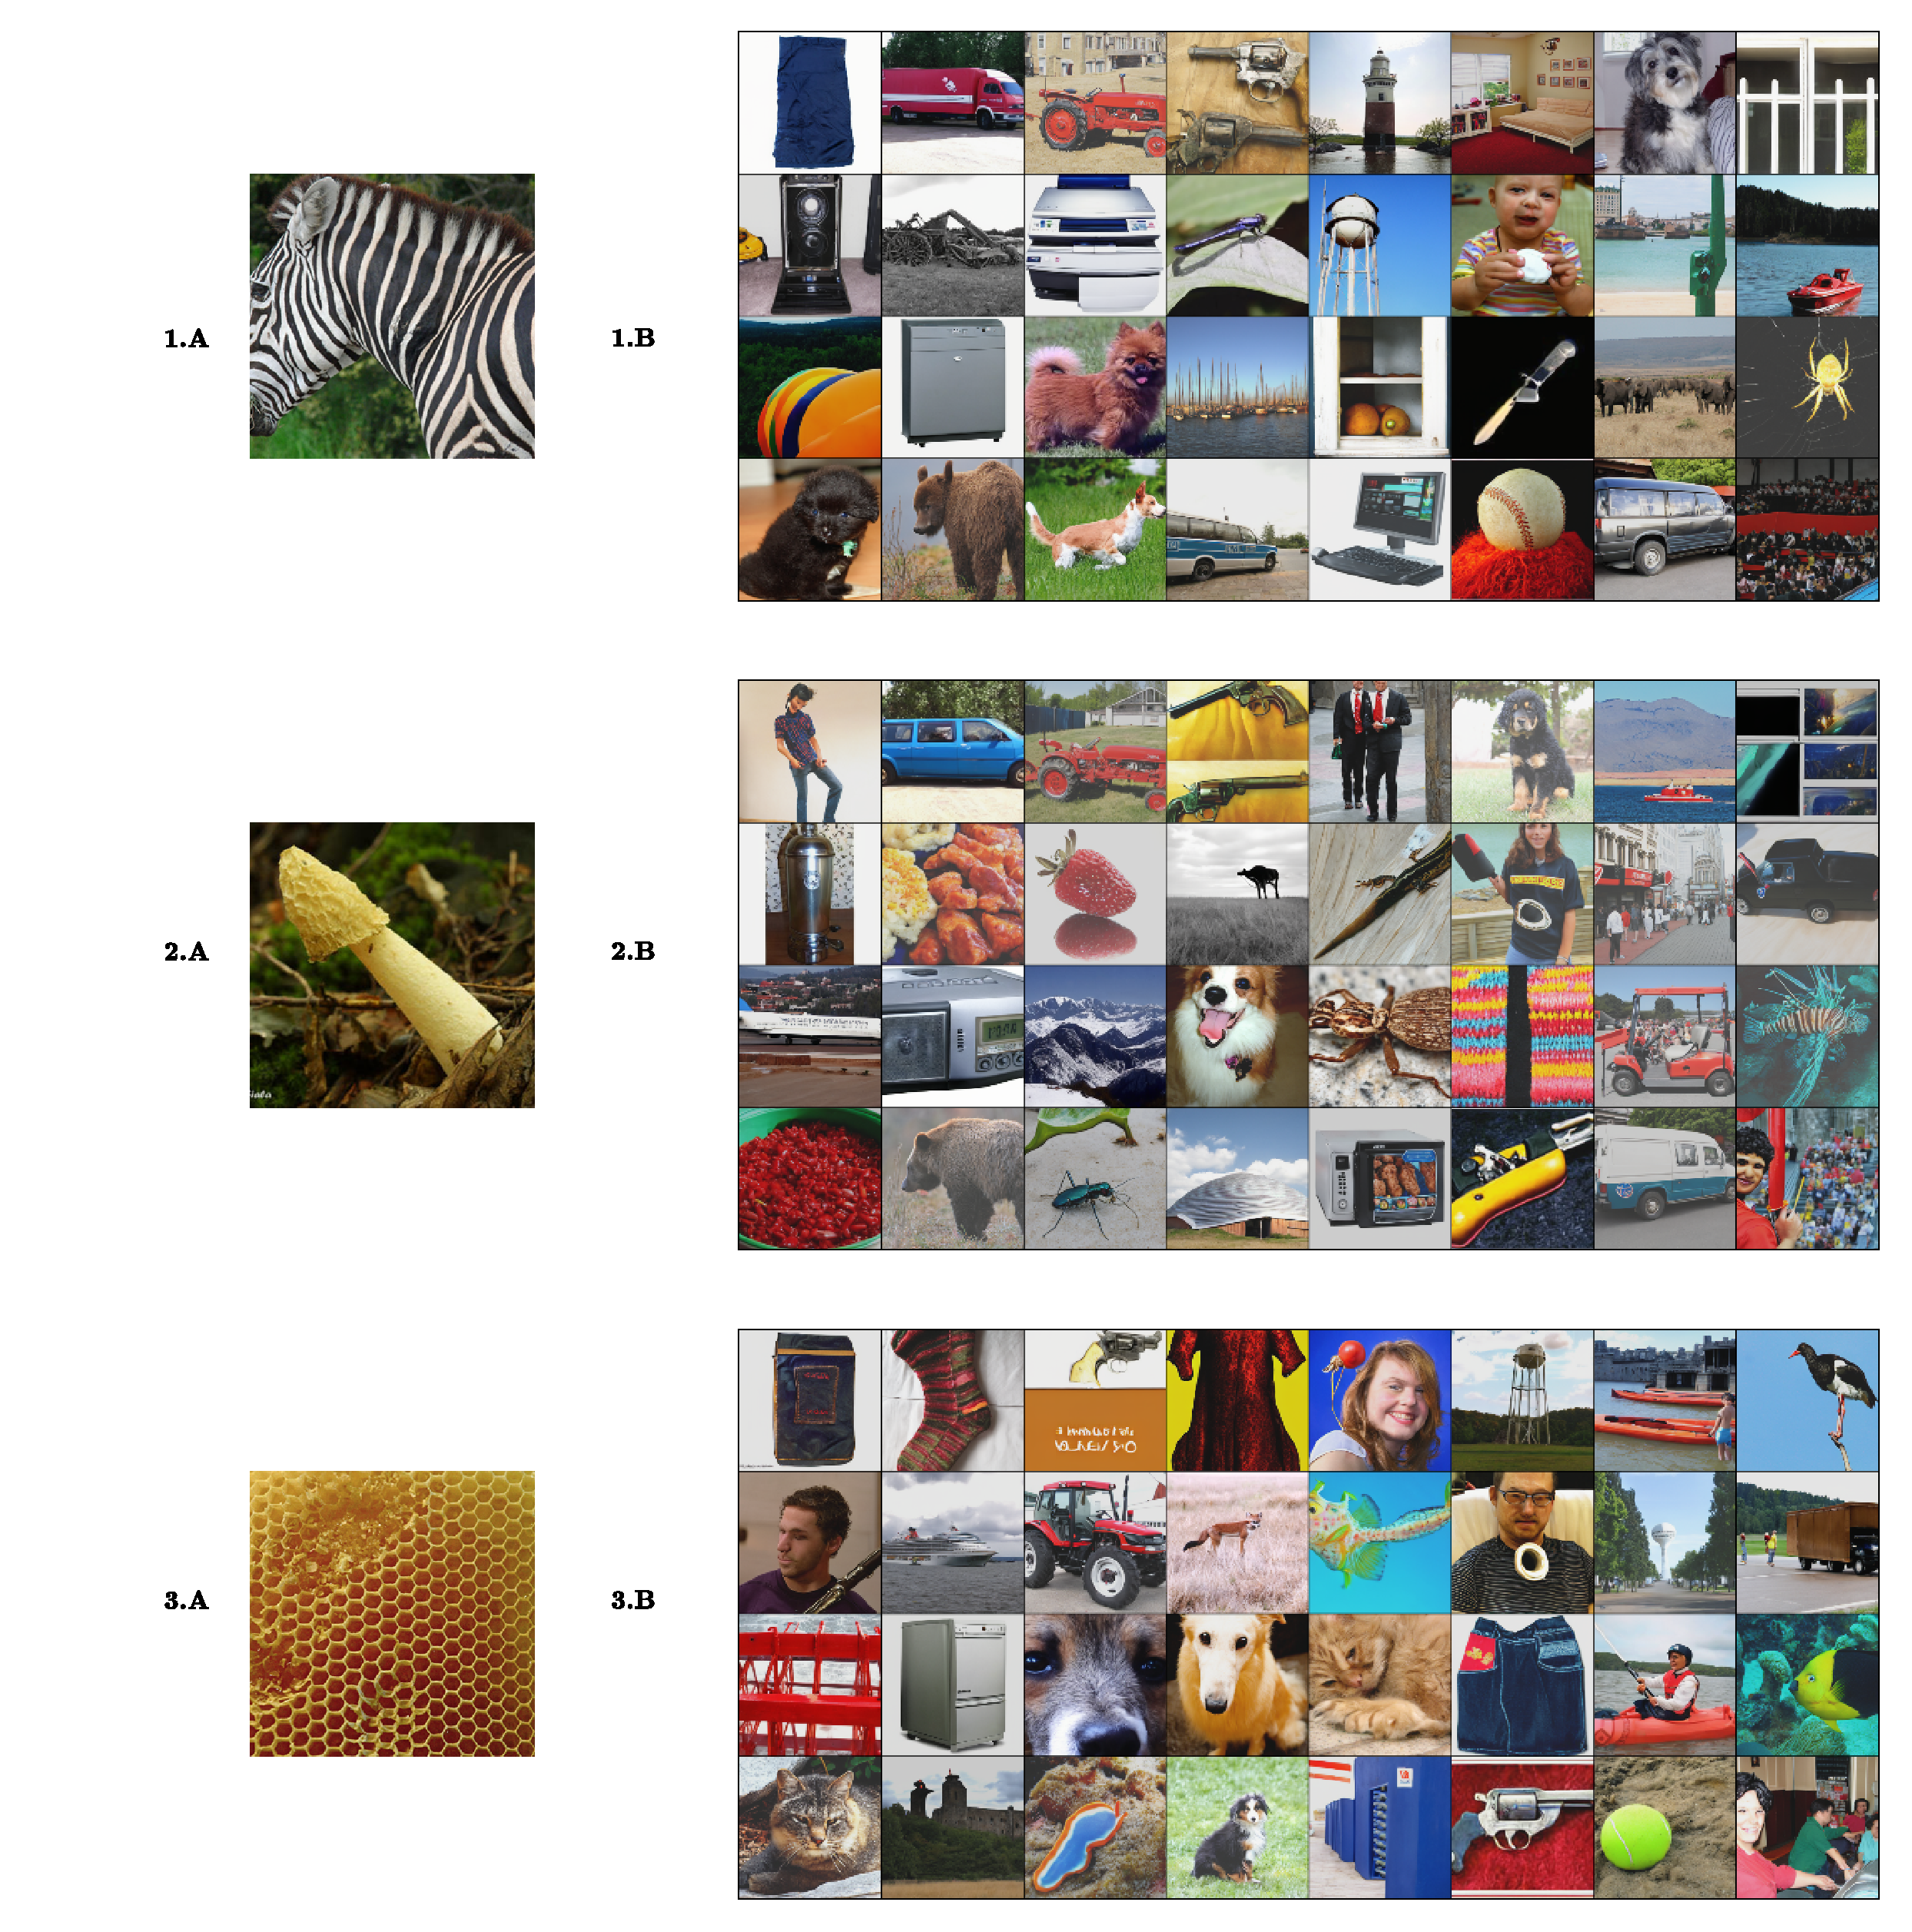
\includegraphics[width=\linewidth]{figures/main/sae_results_1.png}
\caption{ \textbf{B} - Invariant set samples for Neuron \textbf{1}: \#1656 (Zebra Striping), \textbf{2}: \#1052 (Honeycomb), \textbf{3}: \#421 (Gyromitra). \textbf{A} - source images. Generated images demonstrate semantic diversity while maintaining identical activation levels (32 samples, 1024 optimization steps). The method successfully discovers diverse patterns that activate the same neural pathway, revealing the broader scope of visual features detected by this semantic unit.}
\label{fig:experiment_1_1}
\end{figure}

Figure~\ref{fig:experiment_1_1} demonstrates the semantic diversity achieved within the invariant set for targeted neurons. Generated samples exhibit various patterns beyond typical imagery, including architectural elements, textile patterns, and abstract geometric designs, all maintaining identical activation levels.

\subsection{Cross-Neuron Comparison}

The consistent performance across neurons with different semantic specializations (geometric patterns, biological textures, structural elements) demonstrates the generality of our approach. Notably, the inverse relationship between semantic alignment scores and generation difficulty suggests that more specialized neurons provide clearer optimization targets.

\section{Sparse Autoencoder Feature Analysis}

Sparse autoencoders (SAEs) have emerged as powerful tools for decomposing neural network representations into interpretable features. We extend our evaluation to SAE features from Vision Transformer models using the VitPrisma framework \citep{joseph2025prismaopensourcetoolkit}.

\subsection{Experimental Setup}

We target SAE features from ViT models that exhibit clear semantic interpretability:
\begin{itemize}
\item Selection of monosemantic features with high sparsity scores
\item Application of \method{} to preserve specific feature activation patterns
\end{itemize}

\subsection{Expected Results}

Based on our neuron experiments, we anticipate:
\begin{itemize}
\item Successful preservation of SAE feature activations with $L_2$ losses < 1.0
\item Generation of diverse visual patternsv activating identical feature combinations
\end{itemize}

\subsection{Qualitative Results}

Figure~\ref{fig:experiment_1_2} shows representative results for SAE feature \#6547, demonstrating both the precision and semantic richness of our invariant set generation approach. The left panel displays original training images that naturally activate this feature, revealing its learned selectivity.

The generated samples in the top right panel demonstrate remarkable semantic diversity while maintaining mathematical precision in activation preservation (L2 loss $\approx 0.01$). Notably, the generated images extend far beyond the visual patterns present in the original training examples, which are only birds. This expansion of the visual vocabulary suggests that the SAE feature has learned a more abstract and generalizable representation than initially apparent from training data alone.

The qualitative analysis reveals several key insights: (1) the feature exhibits broader semantic scope than suggested by typical training examples, (2) invariant set membership can be maintained across significant stylistic and compositional variations, and (3) our method successfully navigates the high-dimensional space of valid feature activations while preserving visual coherence. These results validate our hypothesis that invariant sets can reveal much fuller representational capacity of learned features, providing a more comprehensive understanding of neural network internal representations than traditional analysis methods based solely on observed training data.


\begin{figure}[h]
\centering
\includegraphics[width=\linewidth]{figures/main/experiment1.2.pdf}
\caption{Invariant set generation for sparse autoencoder feature \#6547 demonstrates precise activation preservation and semantic diversity. \textbf{Left}: Representative real images from the training dataset that naturally activate this feature, establishing the ground truth semantic concept learned by the SAE. \textbf{Top right}: Generated samples from the invariant set using \method{} with 512 optimization steps. All generated images achieve tight activation matching with L2 loss $\approx 0.01$ relative to the target activation level, demonstrating mathematical precision in invariant set membership. The generated samples reveal the broader visual manifold of patterns that trigger identical feature responses, extending beyond the original training examples to include novel compositions, lighting conditions, and stylistic variations while preserving the core semantic concept. This diversity illustrates how invariant sets can expose the full scope of visual patterns encoded by individual SAE features, providing insights into learned representations that extend far beyond observed training data.}
\label{fig:experiment_1_2}
\end{figure}

\section{Classifier Output Preservation}

Our final experimental paradigm evaluates \method{}'s ability to preserve complete classifier outputs, representing the most complex invariant set constraint.

\subsection{Experimental Design}

We investigate invariant set generation for:
\begin{itemize}
\item Single-class prediction preservation (maintaining identical class probabilities)
\item Multi-class logit preservation (preserving full output distributions)  
\end{itemize}

\subsection{Frequency Domain Analysis}

\begin{figure}[h]
\centering
\includegraphics[width=\linewidth]{figures/main/spectral_analysis_1.png}
\caption{Invariant images that preserve ResNet50 classifier probability with ~0.01 L2 loss on the right and original image on the left. Bottom row shows spectral heatmap of the image showing that although generated samples are of high quality but spectral analysis can reveal their synthetic background}
\label{fig:frequency_analysis_1}
\end{figure}

\begin{figure}[h]
\centering
\includegraphics[width=\linewidth]{figures/main/spectral_analysis_2.png}
\caption{Difference between ground true class probability value in source image and in image passed through cut-off filter in spectral domain. This comparison clearly shows that the biggest difference in classifier output occurs around the same frequency value which suggest that although generated samples have different spectral view, they encode signal in the same power levels.}
\label{fig:frequency_analysis_2}
\end{figure}

Figure~\ref{fig:frequency_analysis_2} illustrates our frequency domain evaluation methodology, examining how invariant set membership changes across different spectral bands. This analysis ensures that generated samples achieve invariance through semantically meaningful rather than imperceptible high-frequency variations.

\subsection{Preliminary Observations}

Initial experiments demonstrate:
\begin{itemize}
\item Effective preservation of classification outputs across diverse visual styles
\item Maintenance of prediction confidence levels while varying semantic content  
\item Discovery of unexpected visual patterns yielding identical classifier responses
\end{itemize}

Comprehensive results forthcoming upon experimental completion.

\section{Discussion}

Our experimental evaluation demonstrates \method{}'s effectiveness across multiple scales of neural network analysis, from individual neurons to complete classifier outputs. The consistent achievement of low $L_2$ losses (< 1.0) across different target types indicates robust invariant set preservation, while maintained FID scores confirm generation quality.

\subsection{Key Findings}

\begin{enumerate}
\item \textbf{Precision}: Consistent achievement of tight activation matching across different neural components
\item \textbf{Diversity}: Generation of semantically diverse samples within invariant sets
\item \textbf{Quality}: Maintenance of natural image statistics without adversarial artifacts
\item \textbf{Generality}: Effective performance across different architectures and semantic concepts
\end{enumerate}

\subsection{Limitations and Future Work}

Current limitations include computational expense (limiting sample sizes) and lack of an algorithm to pick the most interesting in some manner members from the Invariant Set. Future work will explore more efficient optimization strategies and extension to other modalities.

The experimental framework established here provides a foundation for systematic evaluation of generative explainability methods, offering both quantitative rigor and qualitative insight into neural network decision-making processes.


\chapter{Applications}\label{r:applications}

\chapter{Discussion}\label{r:discussion}

\chapter{Conclusion}\label{r:conclusion}
\appendix

\section{Infinite Optimization Algorithm}\label{appendix:infinite_optimization}
This appendix provides the detailed algorithmic specification for our invariant set generation method, adapted from the infinite optimization approach. Unlike the original text-conditioned diffusion guidance, our algorithm is specifically designed for generating images that belong to the same invariant set as a given query point.

\begin{algorithm}[H]
\caption{Invariant Set Generation via Infinite Optimization}
\label{alg:invariant_generation}
\begin{algorithmic}[1]
\Require Loss function $\mathcal{L}$, Query point $\mathbf{x^*}$, Target value $\mathcal{L}(\mathbf{x^*})$, Step budget $B$, Loss threshold $\tau$, Learning rate $\eta$, Step size $\lambda$, Low-pass filter $\mathcal{F}$
\Ensure Generated sample $x$ such that $\mathcal{L}(x) \approx \mathcal{L}(\mathbf{x^*})$

\State $z_T \sim \mathcal{N}(0, I)$ \Comment{Draw starting latent}
\State $target\_value = \mathcal{L}(\mathbf{x^*})$ \Comment{Store target invariant value}

\For{$t = 1, \ldots, T$} \Comment{Initialize time step-dependent variables}
    \State $C_t = \emptyset$ \Comment{No conditioning (unconditional generation)}
\EndFor

\State $optim = \text{SGD}(z_T, \text{lr}=\eta)$ \Comment{Define the optimizer}

\State $step\_count = 0$ \Comment{Initialize step counter}
\While{$step\_count < B$} \Comment{Optimization loop with budget}
    \State $z = z_T$ \Comment{Reset to starting latent}
    
    \For{$t = T, \ldots, 1$} \Comment{Denoising loop}
        \State \textbf{with} gradient\_checkpointing():
        \State \quad $z = \text{LightningDiT\_step}(z, t)$ \Comment{Diffusion update according to LightningDiT}
    \EndFor
    
    \State $x = \mathcal{D}(z)$ \Comment{Decode final latent using VAE decoder}
    \State $current\_value = \mathcal{L}(x)$ \Comment{Calculate unfiltered objective value}
    \State $x_{filtered} = \mathcal{F}(x)$ \Comment{Apply low-pass filter}
    \State $current\_value_{filtered} = \mathcal{L}(x_{filtered})$ \Comment{Calculate filtered objective value}
    
    \State $loss_1 = \|current\_value - target\_value\|^2$ \Comment{Unfiltered invariant set loss}
    \State $loss_2 = \|current\_value_{filtered} - target\_value\|^2$ \Comment{Filtered invariant set loss}
    \State $total\_loss = \lambda \cdot (loss_1 + loss_2)$ \Comment{Combined loss with step size}
    
    \If{$total\_loss < \tau$} \Comment{Check convergence threshold}
        \State \textbf{break} \Comment{Early termination}
    \EndIf
    
    \State $total\_loss$.backward() \Comment{Calculate gradients w.r.t. $z_T$}
    
    \State $optim$.step() \Comment{Update starting latent}
    \State $optim$.zero\_grad() \Comment{Clear gradients}
    \State $step\_count = step\_count + 1$ \Comment{Increment step counter}
\EndWhile

\State \Return $z_T$, $x$ \Comment{Return optimized latent and final image}
\end{algorithmic}
\end{algorithm}

\subsection{Key Differences from Original Algorithm}

Our adaptation introduces several important modifications to suit invariant set generation:

\begin{itemize}
    \item \textbf{Unconditional Generation}: Unlike the original text-conditioned approach, we use unconditional diffusion models ($C_t = \emptyset$) and rely entirely on the optimization process to guide generation toward the target invariant set.
    
    \item \textbf{Invariant Set Objective}: Instead of optimizing for text-image alignment, we minimize the $L_2$ distance between $\mathcal{L}(x)$ and the target value $\mathcal{L}(\mathbf{x^*})$, ensuring membership in the same invariant set.
    
    \item \textbf{Frequency Domain Filtering}: We incorporate a low-pass filter $\mathcal{F}$ before computing the objective function to ensure that invariant set membership is achieved through perceptually meaningful variations rather than high-frequency adversarial noise.
    
    \item \textbf{LightningDiT Integration}: The diffusion denoising process follows the LightningDiT sampling procedure, which may use different update rules than standard DDIM depending on the specific implementation and training configuration.
\end{itemize}

\subsection{Computational Considerations}

The infinite optimization approach requires careful management of computational resources:

\begin{itemize}
    \item \textbf{Gradient Checkpointing}: We employ gradient checkpointing during the denoising loop to reduce memory consumption while maintaining gradient flow through the entire diffusion process.
    
    \item \textbf{Optimizer Selection}: Based on empirical evaluation, SGD demonstrates superior convergence properties for invariant set generation compared to adaptive methods like Adam.
    
    \item \textbf{Step Budget Management}: The algorithm balances computational cost with solution quality through the step budget $B$ and threshold $\tau$ parameters, enabling early termination for efficient optimization landscapes.
    
    \item \textbf{Dual Loss Computation}: Computing both filtered and unfiltered objective values provides robustness against adversarial solutions while maintaining semantic coherence in generated samples.
\end{itemize}

\section{Level Set Theory Foundation}\label{appendix:level_sets}

Our \framework{} are mathematically equivalent to level sets from classical analysis. This connection provides theoretical grounding for our generative approach.

\subsection{Basic Definition}

For a function $f: \mathbb{R}^n \rightarrow \mathbb{R}$, the level set at value $c$ is:
\begin{equation}
L_c = \{x \in \mathbb{R}^n : f(x) = c\}
\end{equation}

This is exactly what we compute: all inputs $x$ that produce the same output value $c$.

\subsection{Neural Network Case}

For neural networks outputting vectors $\mathcal{L}_{\boldsymbol{\theta}}: \mathbb{R}^n \rightarrow \mathbb{R}^m$, our invariant sets are intersections of multiple level sets:
\begin{equation}
\mathbf{IS}(\mathbf{x^*}) = \bigcap_{i=1}^m \{x : [\mathcal{L}_{\boldsymbol{\theta}}(x)]_i = [\mathcal{L}_{\boldsymbol{\theta}}(\mathbf{x^*})]_i\}
\end{equation}

Each output dimension defines one level set; we find points lying on all of them simultaneously.

\subsection{Why This Works}

Level sets typically form smooth geometric surfaces when the function gradients are non-zero. Our diffusion model samples from these surfaces while staying within the natural image manifold. This geometric perspective explains why we can generate diverse yet valid samples from invariant sets.

\section{Implementation Details}\label{appendix:implementation}

This section provides the specific implementation parameters used throughout our experiments.

\subsection{Optimization Configuration}

Based on empirical evaluation, we selected:
\begin{itemize}
\item \textbf{Optimizer}: SGD (most stable convergence)
\item \textbf{Learning Rate}: $\eta = 10$ (optimal balance of speed and stability)
\item \textbf{Step Budget}: 512 or 1024 steps (sufficient for convergence)
\item \textbf{Loss Threshold}: $\tau = 0.01$ (tight precision requirement for early stopping)
\end{itemize}

\subsection{Hardware Configuration}

All experiments conducted on:
\begin{itemize}
\item NVIDIA A100 GPUs (1-4 units depending on experiment)
\item PyTorch framework with CUDA most recent  acceleration such as Flash Attention \citep{dao2022flashattention, dao2023flashattention2}
\item Gradient checkpointing for memory efficiency
\end{itemize}

\section{Frequency Domain Analysis}\label{appendix:frequency_analysis}

Our spectral analysis ensures that invariant set membership relies on semantic rather than imperceptible features.

\subsection{Filter Implementation}

We apply ideal low-pass filters in frequency domain:
\begin{equation}
\mathcal{F}_{cutoff}(\mathbf{x}) = \mathcal{F}^{-1}(\mathbf{H}_{cutoff} \cdot \mathcal{F}(\mathbf{x}))
\end{equation}

where $\mathbf{H}_{cutoff}$ removes frequencies beyond the cutoff threshold.

\subsection{Analysis Protocol}

For each generated sample, we:
\begin{enumerate}
\item Apply filters with cutoffs from 0.1 to 0.9
\item Compute network response on filtered images
\item Measure deviation from target response
\item Plot spectral preservation across frequency bands
\end{enumerate}

\subsection{Quality Interpretation}

Low deviations at high cutoff values indicate that invariance is preserved even when fine details are removed, confirming semantic rather than adversarial invariance.

\section{Neuron Selection Methodology}\label{appendix:neuron_selection}

We selected interpretable neurons using the Semantic Lens framework \citep{dreyer2025mechanisticunderstandingvalidationlarge}.

\subsection{Selection Criteria}

Neurons were chosen based on:
\begin{itemize}
\item \textbf{Semantic Alignment}: Score $r > 0.85$ (high interpretability)
\item \textbf{Concept Clarity}: Clear, consistent activation patterns
\item \textbf{Diversity}: Different semantic categories (geometric, biological, textural)
\end{itemize}

\subsection{Selected Neurons}

Our three target neurons:
\begin{itemize}
\item \textbf{Neuron \#1656}: Zebra striping patterns ($r = 0.945$)
\item \textbf{Neuron \#1052}: Honeycomb structures ($r = 0.880$)
\item \textbf{Neuron \#421}: Gyromitra morphology ($r = 0.952$)
\end{itemize}

These represent well-understood, semantically interpretable units with high activation specificity.

\bibliography{references}

\end{document}


%%% Local Variables:
%%% mode: latex
%%% TeX-master: t
%%% coding: latin-2
%%% End:
